\documentclass[10pt,xcolor={dvipsnames}]{beamer}
\usepackage[utf8]{inputenc}
\usepackage{graphicx}

\usetheme{Copenhagen}
\usecolortheme{seagull}

\usepackage{caption}
\usepackage{media9}
% \usepackage{media9}%
\newcommand{\includemovie}[3]{%
\includemedia[%
width=#1,height=#2,%
activate=pagevisible,%
deactivate=pageclose,%
addresource=#3,%
flashvars={%
src=#3 % same path as in addresource!
&autoPlay=true % default: false; if =true, automatically starts playback after activation (see option ‘activation)’
&loop=true % if loop=true, media is played in a loop
&controlBarAutoHideTimeout=0 %  time span before auto-hide
}%
]{}{StrobeMediaPlayback.swf}%
}% end of the new command

\usepackage{booktabs,siunitx}
\usepackage{multirow}
\usepackage[flushleft]{threeparttable}


\usepackage{amsmath}
\usepackage{stmaryrd}

\usepackage{amssymb}% http://ctan.org/pkg/amssymb
\usepackage{pifont}% http://ctan.org/pkg/pifont

\usepackage{animate}
\usepackage{adjustbox}

\usepackage{tikz}
\usepackage{amsfonts}
\usepackage{xcolor}
\usepackage{biblatex}
\usepackage{hyperref}
\usetikzlibrary{shapes,
                tikzmark}
\tikzset{every tikzmarknode/.style={%
        draw=red, semithick, inner sep=2pt}
        % invisible/.style={opacity=0},
        % tikzmarknode/.style={opacity=1},
        % alt/.code args={<#1>#2#3}{%
        % \alt<#1>{\pgfkeysalso{#2}}{\pgfkeysalso{#3}} % \pgfkeysalso doesn't change the path
        % },
        }

\tiny\bibliography{references.bib}
\usetikzlibrary{calc}
\DeclareMathOperator*{\argmax}{arg\,max}
\DeclareMathOperator*{\argmin}{arg\,min}
\DeclareMathOperator*{\argminB}{argmin}

\definecolor{red}{rgb}{1.00,0.00,0.00}
\definecolor{blue}{rgb}{0.00,0.00,1.00}
\definecolor{dblue}{rgb}{0.00,0.00,0.40}
\definecolor{green}{rgb}{0.4,1.00,0.0}
\definecolor{dgreen}{rgb}{0.0,0.40,0.0}
\definecolor{yellow}{rgb}{0.5,0.5,0.0}

%\renewcommand<>{\item}[1]{\only#2{\beameroriginal{\item}{#1}}}


%%%%%%%%%%%%%%%%%%%%%%%%%%%%%%%%%%%%%%%%%%%%%%%%%%%%%%%%%%%%%%%%%%%%%%%%%%%%%%%%%%%%%%%%%%%%%%%%%%%%%%%%%%%%%%%%%%%%%%%%---
%This block of code defines the information to appear in the
%Title page
\title[]
{\large Start Together - PDEM}

\subtitle{}

\author[Joel Baptista] % (optional)
{Joel Baptista}

\institute[VFU] % (optional)
{
  \inst{1}%
  Department of Mechanical Engineering\\
  University of Aveiro, Portugal
  \and
  \inst{2}%
  Institute of Electronics and Informatics Engineering of Aveiro\\
  University of Aveiro, Portugal

}

\date[2025/09/15] % (optional)
{15/09/2025}


\titlegraphic{\begin{center}
\begin{tabular}{c}
%\includegraphics[height=1cm]{img/cytedlogo} &

\includegraphics[height=1cm]{img/Logo-UA-300x300} 
\end{tabular}
\end{center}
}

\setbeamertemplate{footline}[frame number]
\setbeamertemplate{navigation symbols}{}

%End of title page configuration block
%%%%%%%%%%%%%%%%%%%%%%%%%%%%%%%%%%%%%%%%%%%%%%%%%%%%%%%%%%%%%%%%%%%%%%%%%%%%%%%%%%%%%%%%%%%%%%%%%%%%%%%%%%%%%%%%%%%%%%%%---



%%%%%%%%%%%%%%%%%%%%%%%%%%%%%%%%%%%%%%%%%%%%%%%%%%%%%%%%%%%%%%%%%%%%%%%%%%%%%%%%%%%%%%%%%%%%%%%%%%%%%%%%%%%%%%%%%%%%%%%%---
%The next block of commands puts the table of contents at the 
%beginning of each section and highlights the current section:

% \AtBeginSection[]
% {
%   \begin{frame}
%     \frametitle{Table of Contents}
%     \tableofcontents[currentsection]
%   \end{frame}
% }
%%%%%%%%%%%%%%%%%%%%%%%%%%%%%%%%%%%%%%%%%%%%%%%%%%%%%%%%%%%%%%%%%%%%%%%%%%%%%%%%%%%%%%%%%%%%%%%%%%%%%%%%%%%%%%%%%%%%%%%%---


\begin{document}

%The next statement creates the title page.
\frame{\titlepage}


%%%%%%%%%%%%%%%%%%%%%%%%%%%%%%%%%%%%%%%%%%%%%%%%%%%%%%%%%%%%%%%%%%%%%%%%%%%%%%%%%%%%%%%%%%%%%%%%%%%%%%%%%%%%%%%%%%%%%%%%
%This block of code is for the table of contents after
%the title page

%%%%%%%%%%%%%%%%%%%%%%%%%%%%%%%%%%%%%%%%%%%%%%%%%%%%%%%%%%%%%%%%%%%%%%%%%%%%%%%%%%%%%%%%%%%%%%%%%%%%%%%%%%%%%%%%%%%%%%%%
\section{Introduction}
% %%%%%%%%%%%%%%%%%%%%%%%%%%%%%%%%%%%%%%%%%%%%%%%%%%%%%%%%%%%%%%%%%%%%%%%%%%%%%%%%%%%%%%%%%%%%%%%%%%%%%%%%%%%%%%%%%%%%%%%%%
\subsection{Focus}
%%%%%%%%%%%%%%%%%%%%%%%%%%%%%%%%%%%%%%%%%%%%%%%%%%%%%%%%%%%%%%%%%%%%%%%%%%%%%%%%%%%%%%%%%%%%%%%%%%%%%%%%%%%%%%%%%%%%%%%%%

%%%%%%%%%%%%%%%%%%%%%%%%%%%%%%%%%%%%%%%%%%%%%%%%%%%%%%%%%%%%%%%%%%%%%%%%%%%%%%%%%%%%%%%%%%%%%%%%%%%%%%%%%%%%%%%%%%%%%%%%%
\begin{frame}{Focus}
  \begin{figure}
    \centering
    
\includegraphics[width=\textwidth]{img/title.png}
  \end{figure}
  \pause
  Translation: Explore different learning methodologies to create intelligent agents that can control robots in difficult tasks
\end{frame}
%%%%%%%%%%%%%%%%%%%%%%%%%%%%%%%%%%%%%%%%%%%%%%%%%%%%%%%%%%%%%%%%%%%%%%%%%%%%%%%%%%%%%%%%%%%%%%%%%%%%%%%%%%%%%%%%%%%%%%%%
\begin{frame}{Focus}
  \begin{figure}
    \centering
    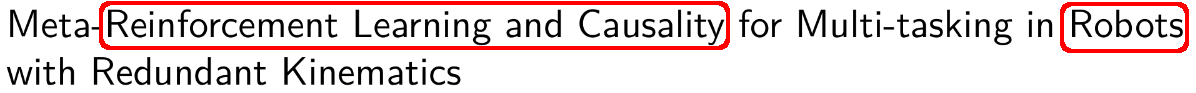
\includegraphics[width=\textwidth]{img/title_annotated.png}
  \end{figure}
  Translation: Explore different learning methodologies to create intelligent agents that can control robots in difficult tasks
\end{frame}
%%%%%%%%%%%%%%%%%%%%%%%%%%%%%%%%%%%%%%%%%%%%%%%%%%%%%%%%%%%%%%%%%%%%%%%%%%%%%%%%%%%%%%%%%%%%%%%%%%%%%%%%%%%%%%%%%%%%%%%%%
\subsection{Motivation}
%%%%%%%%%%%%%%%%%%%%%%%%%%%%%%%%%%%%%%%%%%%%%%%%%%%%%%%%%%%%%%%%%%%%%%%%%%%%%%%%%%%%%%%%%%%%%%%%%%%%%%%%%%%%%%%%%%%%%%%%%
\begin{frame}{Motivation}
  \begin{figure}
    \centering
    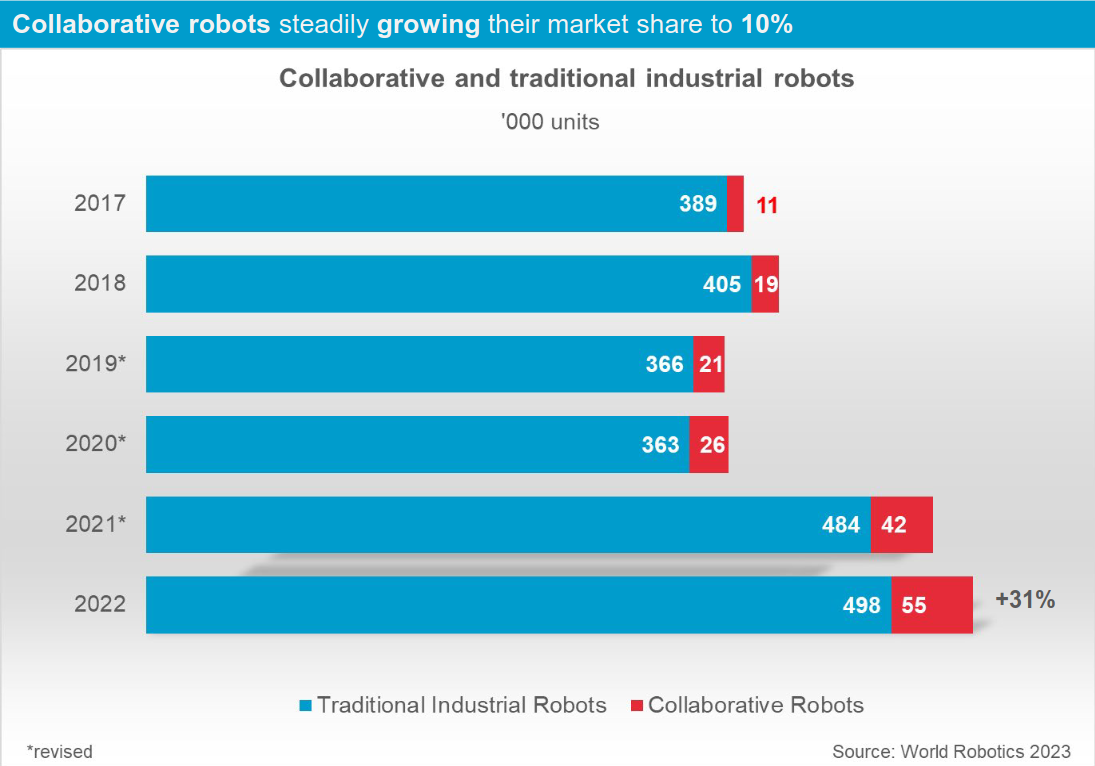
\includegraphics[width=0.7\textwidth]{img/cobot_hist.png}
    \caption{Collaborative and traditional industrial robots' growth\footnotemark}
  \end{figure}
  \footnotetext[1]{Source: \href{https://ifr.org/img/worldrobotics/2023_WR_extended_version.pdf}{World Robotics Report 2023 - Press Conference} }
\end{frame}
%%%%%%%%%%%%%%%%%%%%%%%%%%%%%%%%%%%%%%%%%%%%%%%%%%%%%%%%%%%%%%%%%%%%%%%%%%%%%%%%%%%%%%%%%%%%%%%%%%%%%%%%%%%%%%%%%%%%%%%%%
\begin{frame}{Motivation}
  \begin{figure}[ht]
    \begin{minipage}[b]{0.49\linewidth}
        \centering
        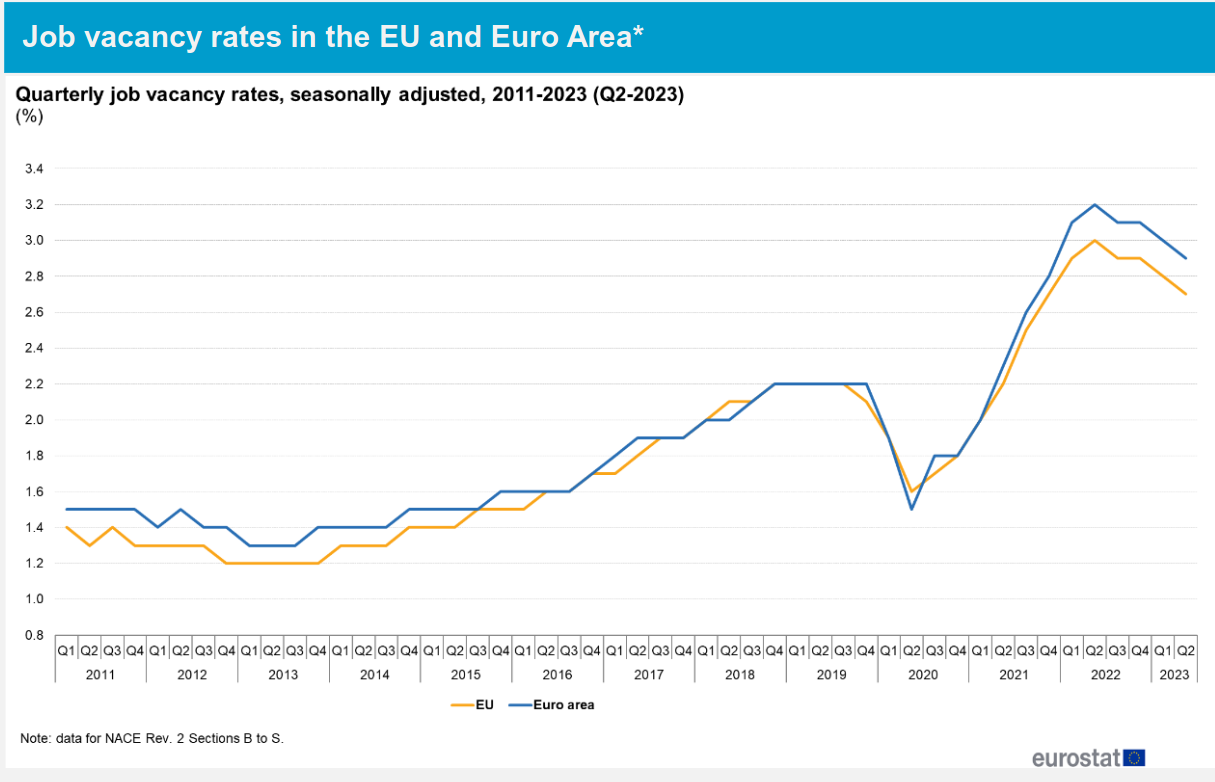
\includegraphics[width=\textwidth, height=0.7\textwidth]{img/job_vacancy.png}
    \end{minipage}
    \begin{minipage}[b]{0.49\linewidth}
        \centering
        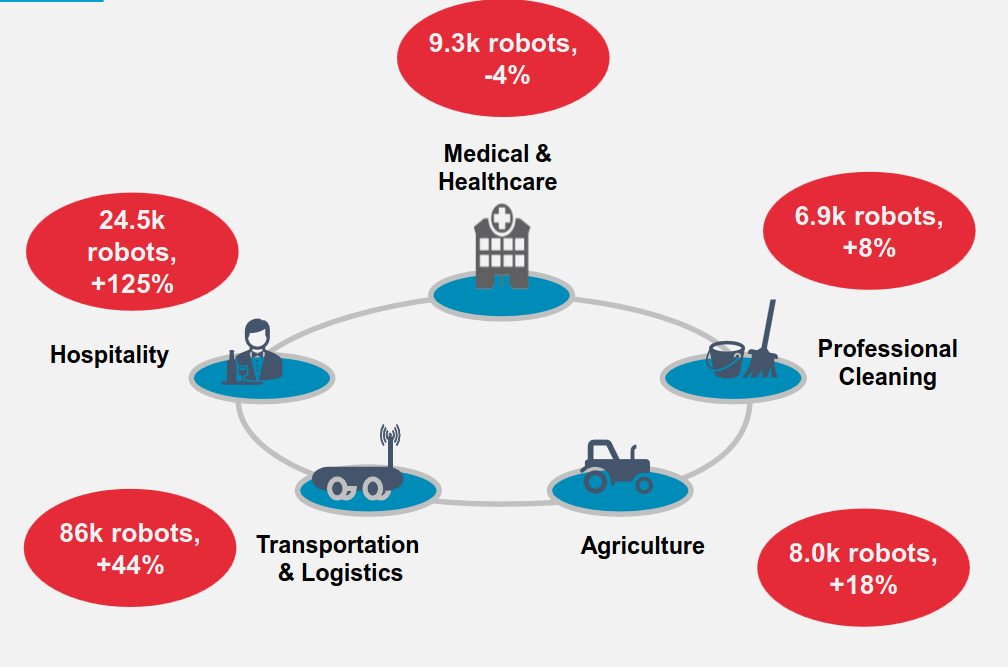
\includegraphics[width=\textwidth]{img/service_robots.png}
    \end{minipage}
    \caption{Job vacancy and service robots' growth\footnotemark[1]}
  \end{figure}
  Job vacancy is rising and the field of service robots is growing in response
  
  \footnotetext[1]{Source: \href{https://ifr.org/img/worldrobotics/2023_WR_extended_version.pdf}{World Robotics Report 2023 - Press Conference} }
\end{frame}
%%%%%%%%%%%%%%%%%%%%%%%%%%%%%%%%%%%%%%%%%%%%%%%%%%%%%%%%%%%%%%%%%%%%%%%%%%%%%%%%%%%%%%%%%%%%%%%%%%%%%%%%%%%%%%%%%%%%%%%%%
\begin{frame}{Motivation}
  Cobots and Service Robots interact in more complex and uncontrolled environments, ...

  \pause
  ... therefore, they need to be more \textbf{\underline{flexible and adaptable}} to different tasks.

\end{frame}
%%%%%%%%%%%%%%%%%%%%%%%%%%%%%%%%%%%%%%%%%%%%%%%%%%%%%%%%%%%%%%%%%%%%%%%%%%%%%%%%%%%%%%%%%%%%%%%%%%%%%%%%%%%%%%%%%%%%%%%%%

\section{The first year}
\begin{frame}{Multitask SACAAR}
    \begin{figure}
        \begin{minipage}[t]{0.45\linewidth}
            \centering
            \vspace{0pt}
            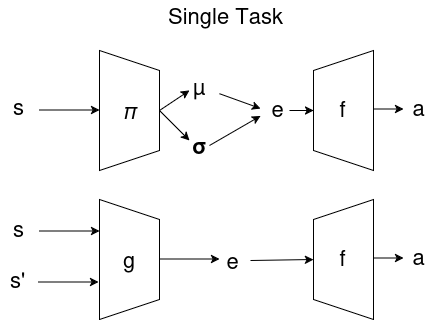
\includegraphics[width=\textwidth]{img/single_task_sacaar.png}
        \end{minipage}
        \hspace{0.5cm}
        \begin{minipage}[t]{0.45\linewidth}
            \centering
            \vspace{0pt}
            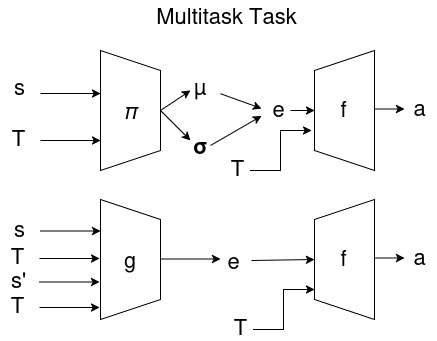
\includegraphics[width=\textwidth]{img/multi_task_sacaar.png}
        \end{minipage}
    \end{figure}
\end{frame}
\begin{frame}{Ànalise do vector condicionante de tarefa}
    \begin{figure}
        \centering
        \vspace{0pt}
        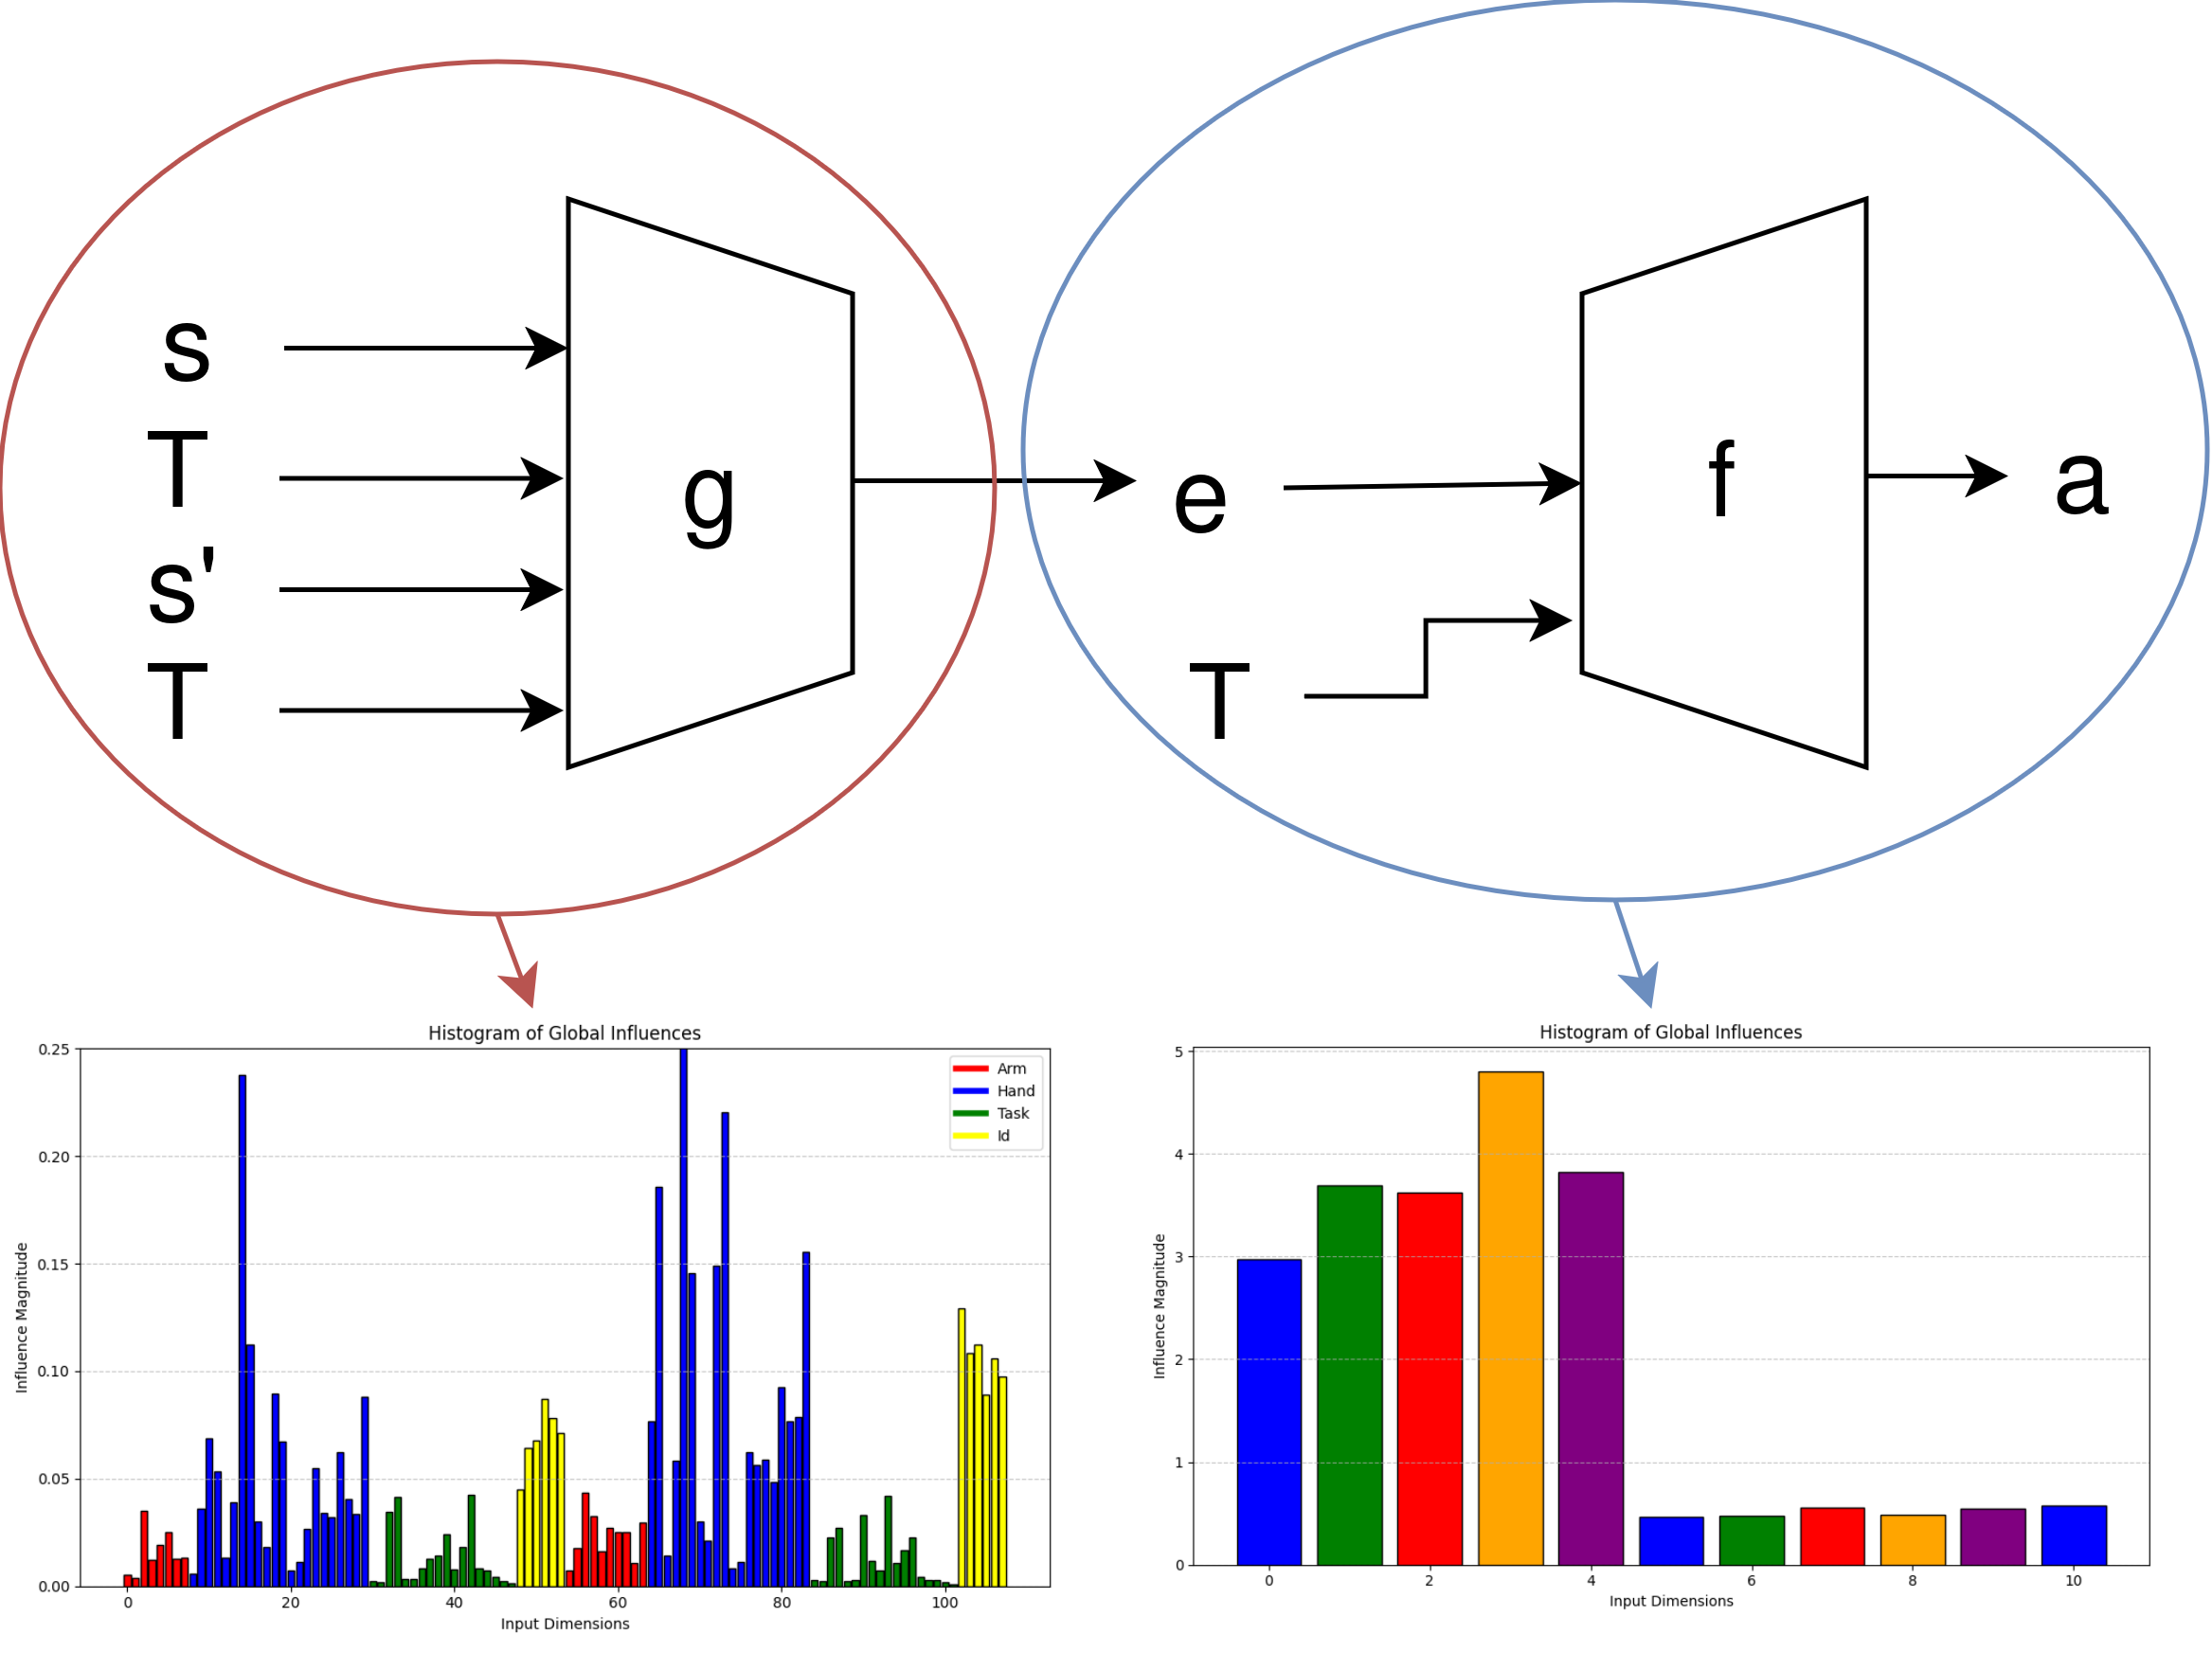
\includegraphics[width=0.7\textwidth]{img/sacaar_ig.png}
    \end{figure}
\end{frame}
\begin{frame}{Potenciais problemas}
    \begin{figure}
        \begin{minipage}[t]{0.4\linewidth}
            \centering
            \vspace{0pt}
            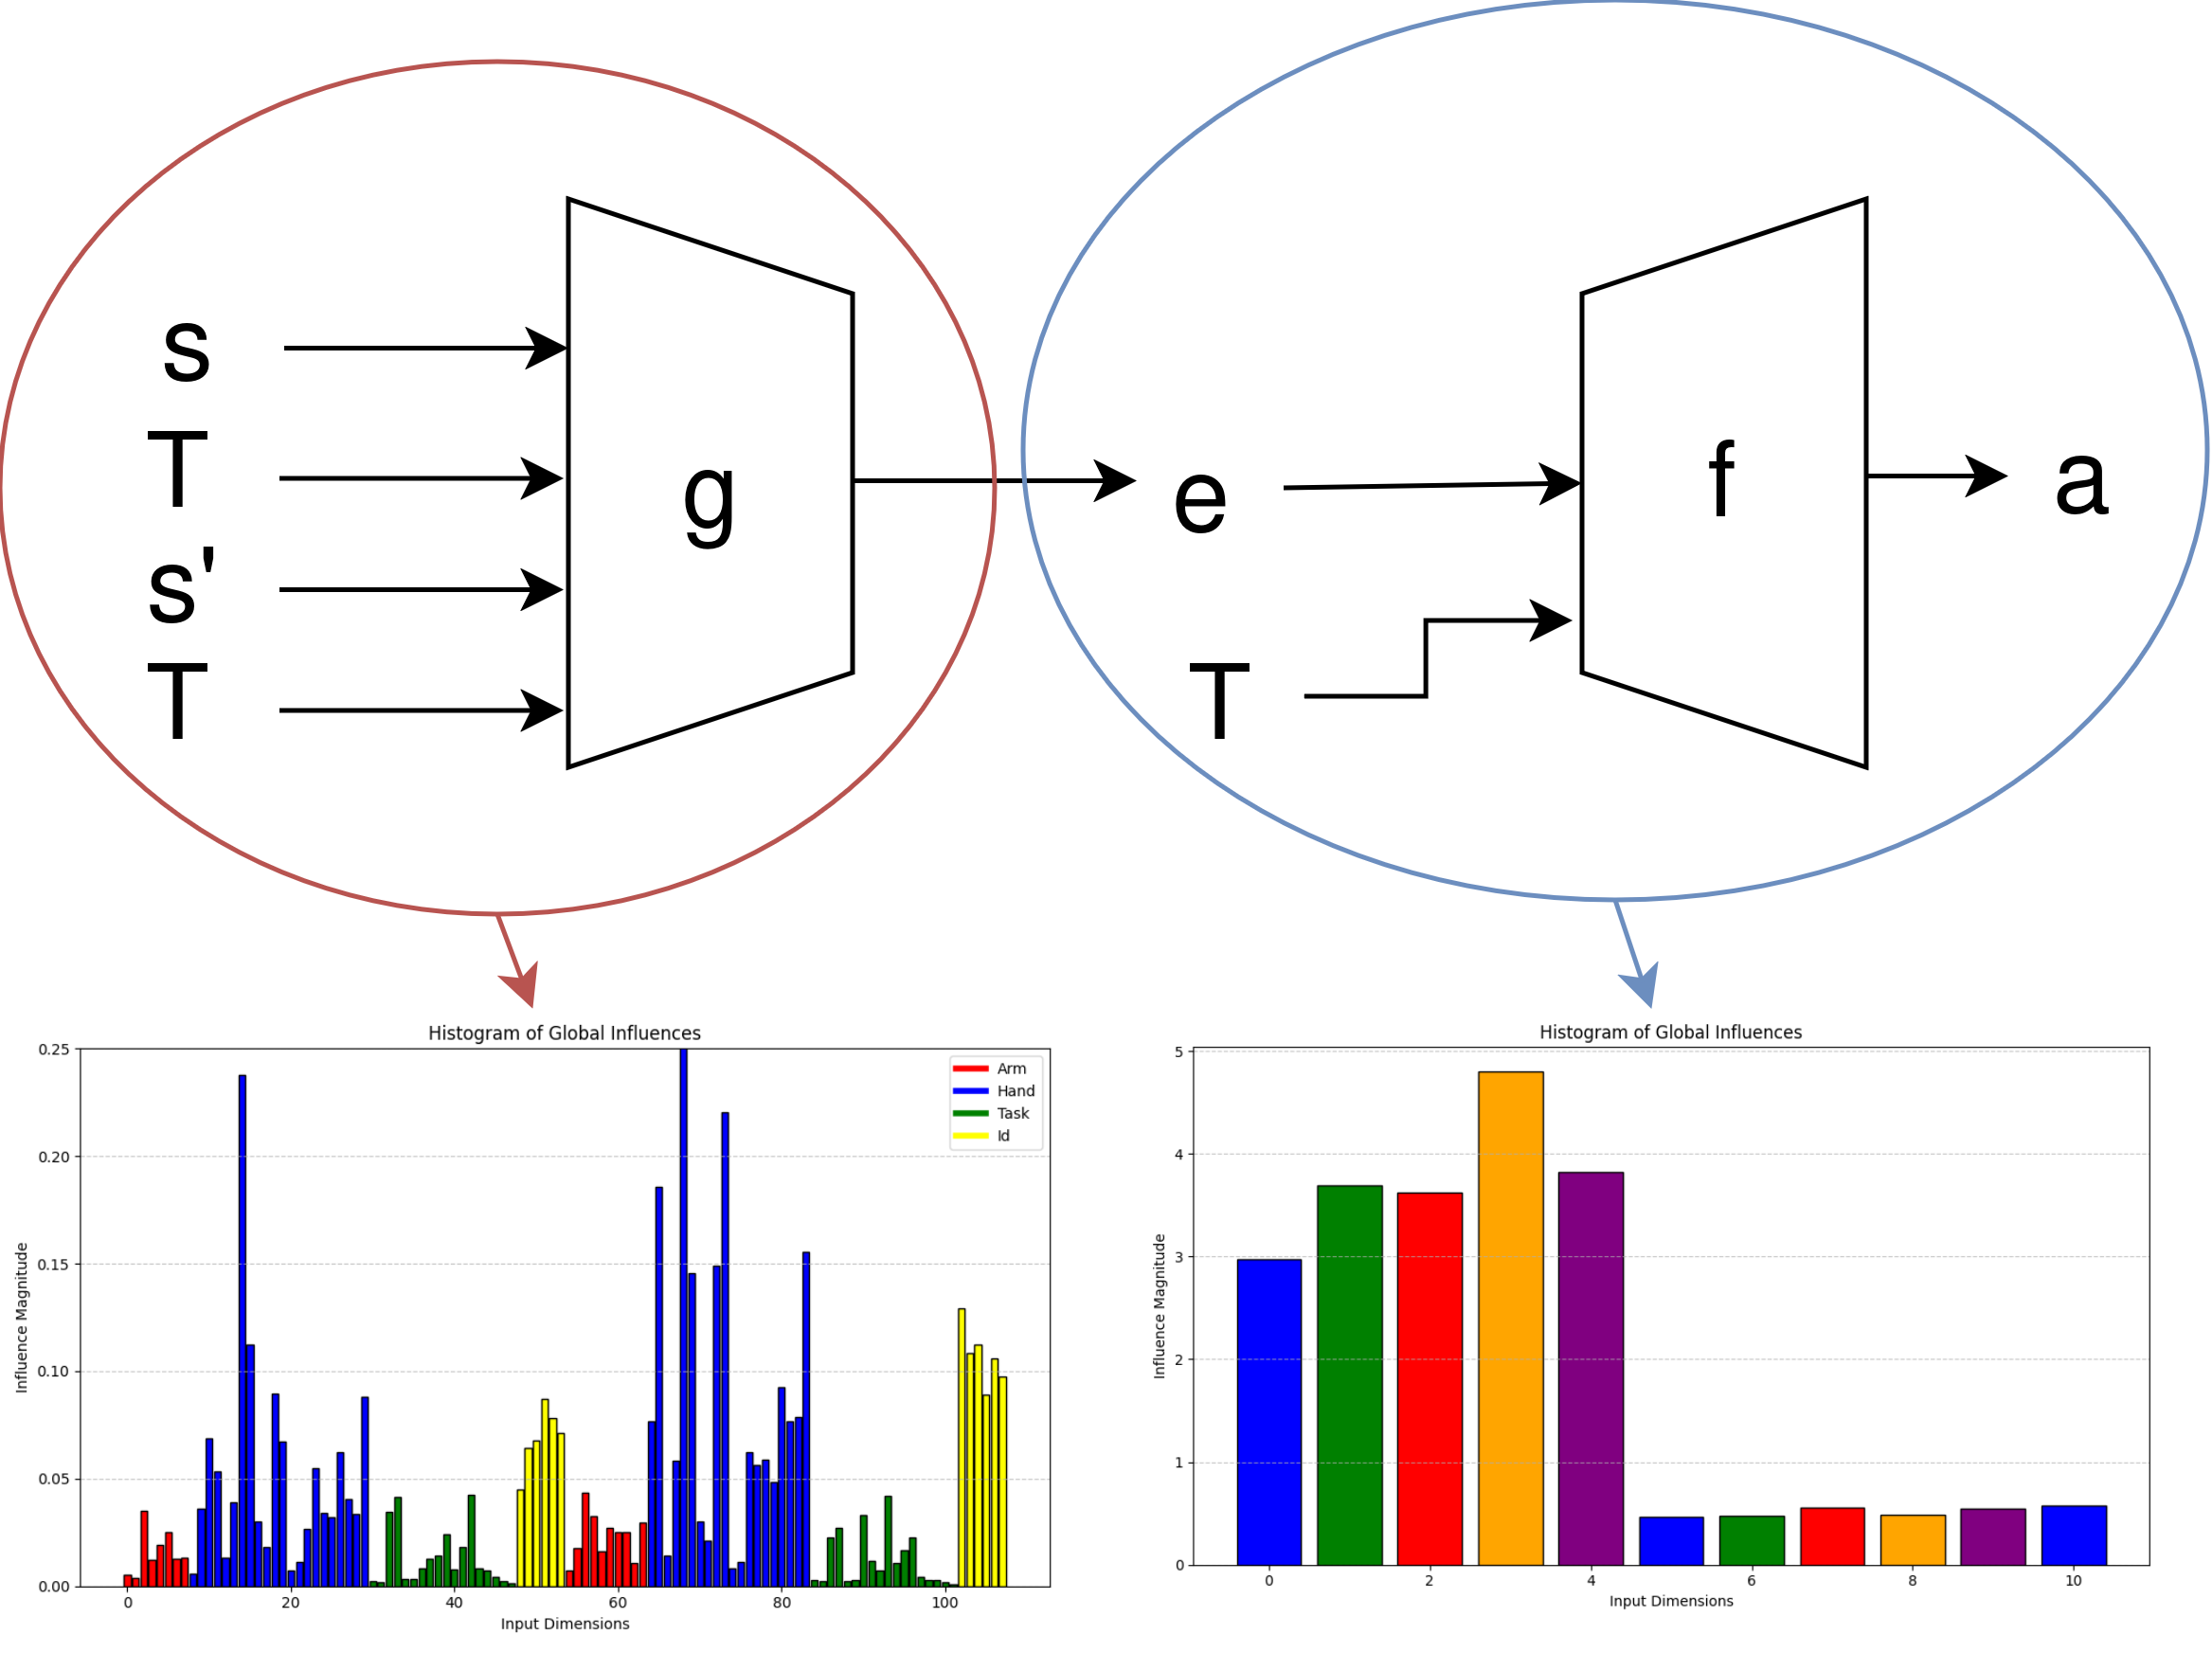
\includegraphics[width=\textwidth]{img/sacaar_ig.png}
        \end{minipage}
        \hspace{0.5cm}
        \begin{minipage}[t]{0.4\linewidth}
            \begin{itemize}
                \item Codificação one-hot (e.g. [1, 0, 0]) é demasiado esparsa.
                \item Informação da tarefa vem do input do encoder e é ignorada no condicionamento
                \item As ações no dataset são independente das ações
            \end{itemize}
        \end{minipage}
    \end{figure}
\end{frame}
\begin{frame}{Problema 1}
    Problema: Codificação one-hot (e.g. [1, 0, 0]) é demasiado esparsa.

    Solução: Utilizar um modelo que adquirir um vector de tarefa com valor mais continuo 

    \begin{figure}
        \begin{minipage}[t]{0.45\linewidth}
            \centering
            \vspace{0pt}
            
\includegraphics[width=\textwidth]{img/task_encoder.png}
        \end{minipage}
        \hspace{0.5cm}
        \begin{minipage}[t]{0.45\linewidth}
            \centering
            \vspace{0pt}
            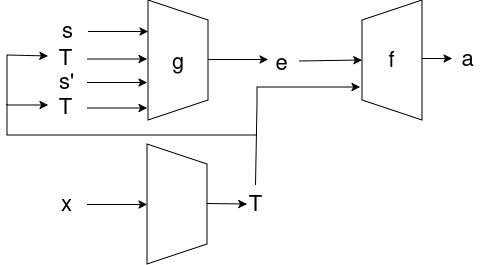
\includegraphics[width=\textwidth]{img/sacaar_encoded.png}
        \end{minipage}
    \end{figure}
\end{frame}
\begin{frame}{Problema 2}
    Problema: Informação da tarefa vem do input do encoder e é ignorada no condicionamento.

    Solução: Retirar a informação da tarefa do input do modelo de representação 

    \begin{figure}
        \centering
        \vspace{-10pt}
        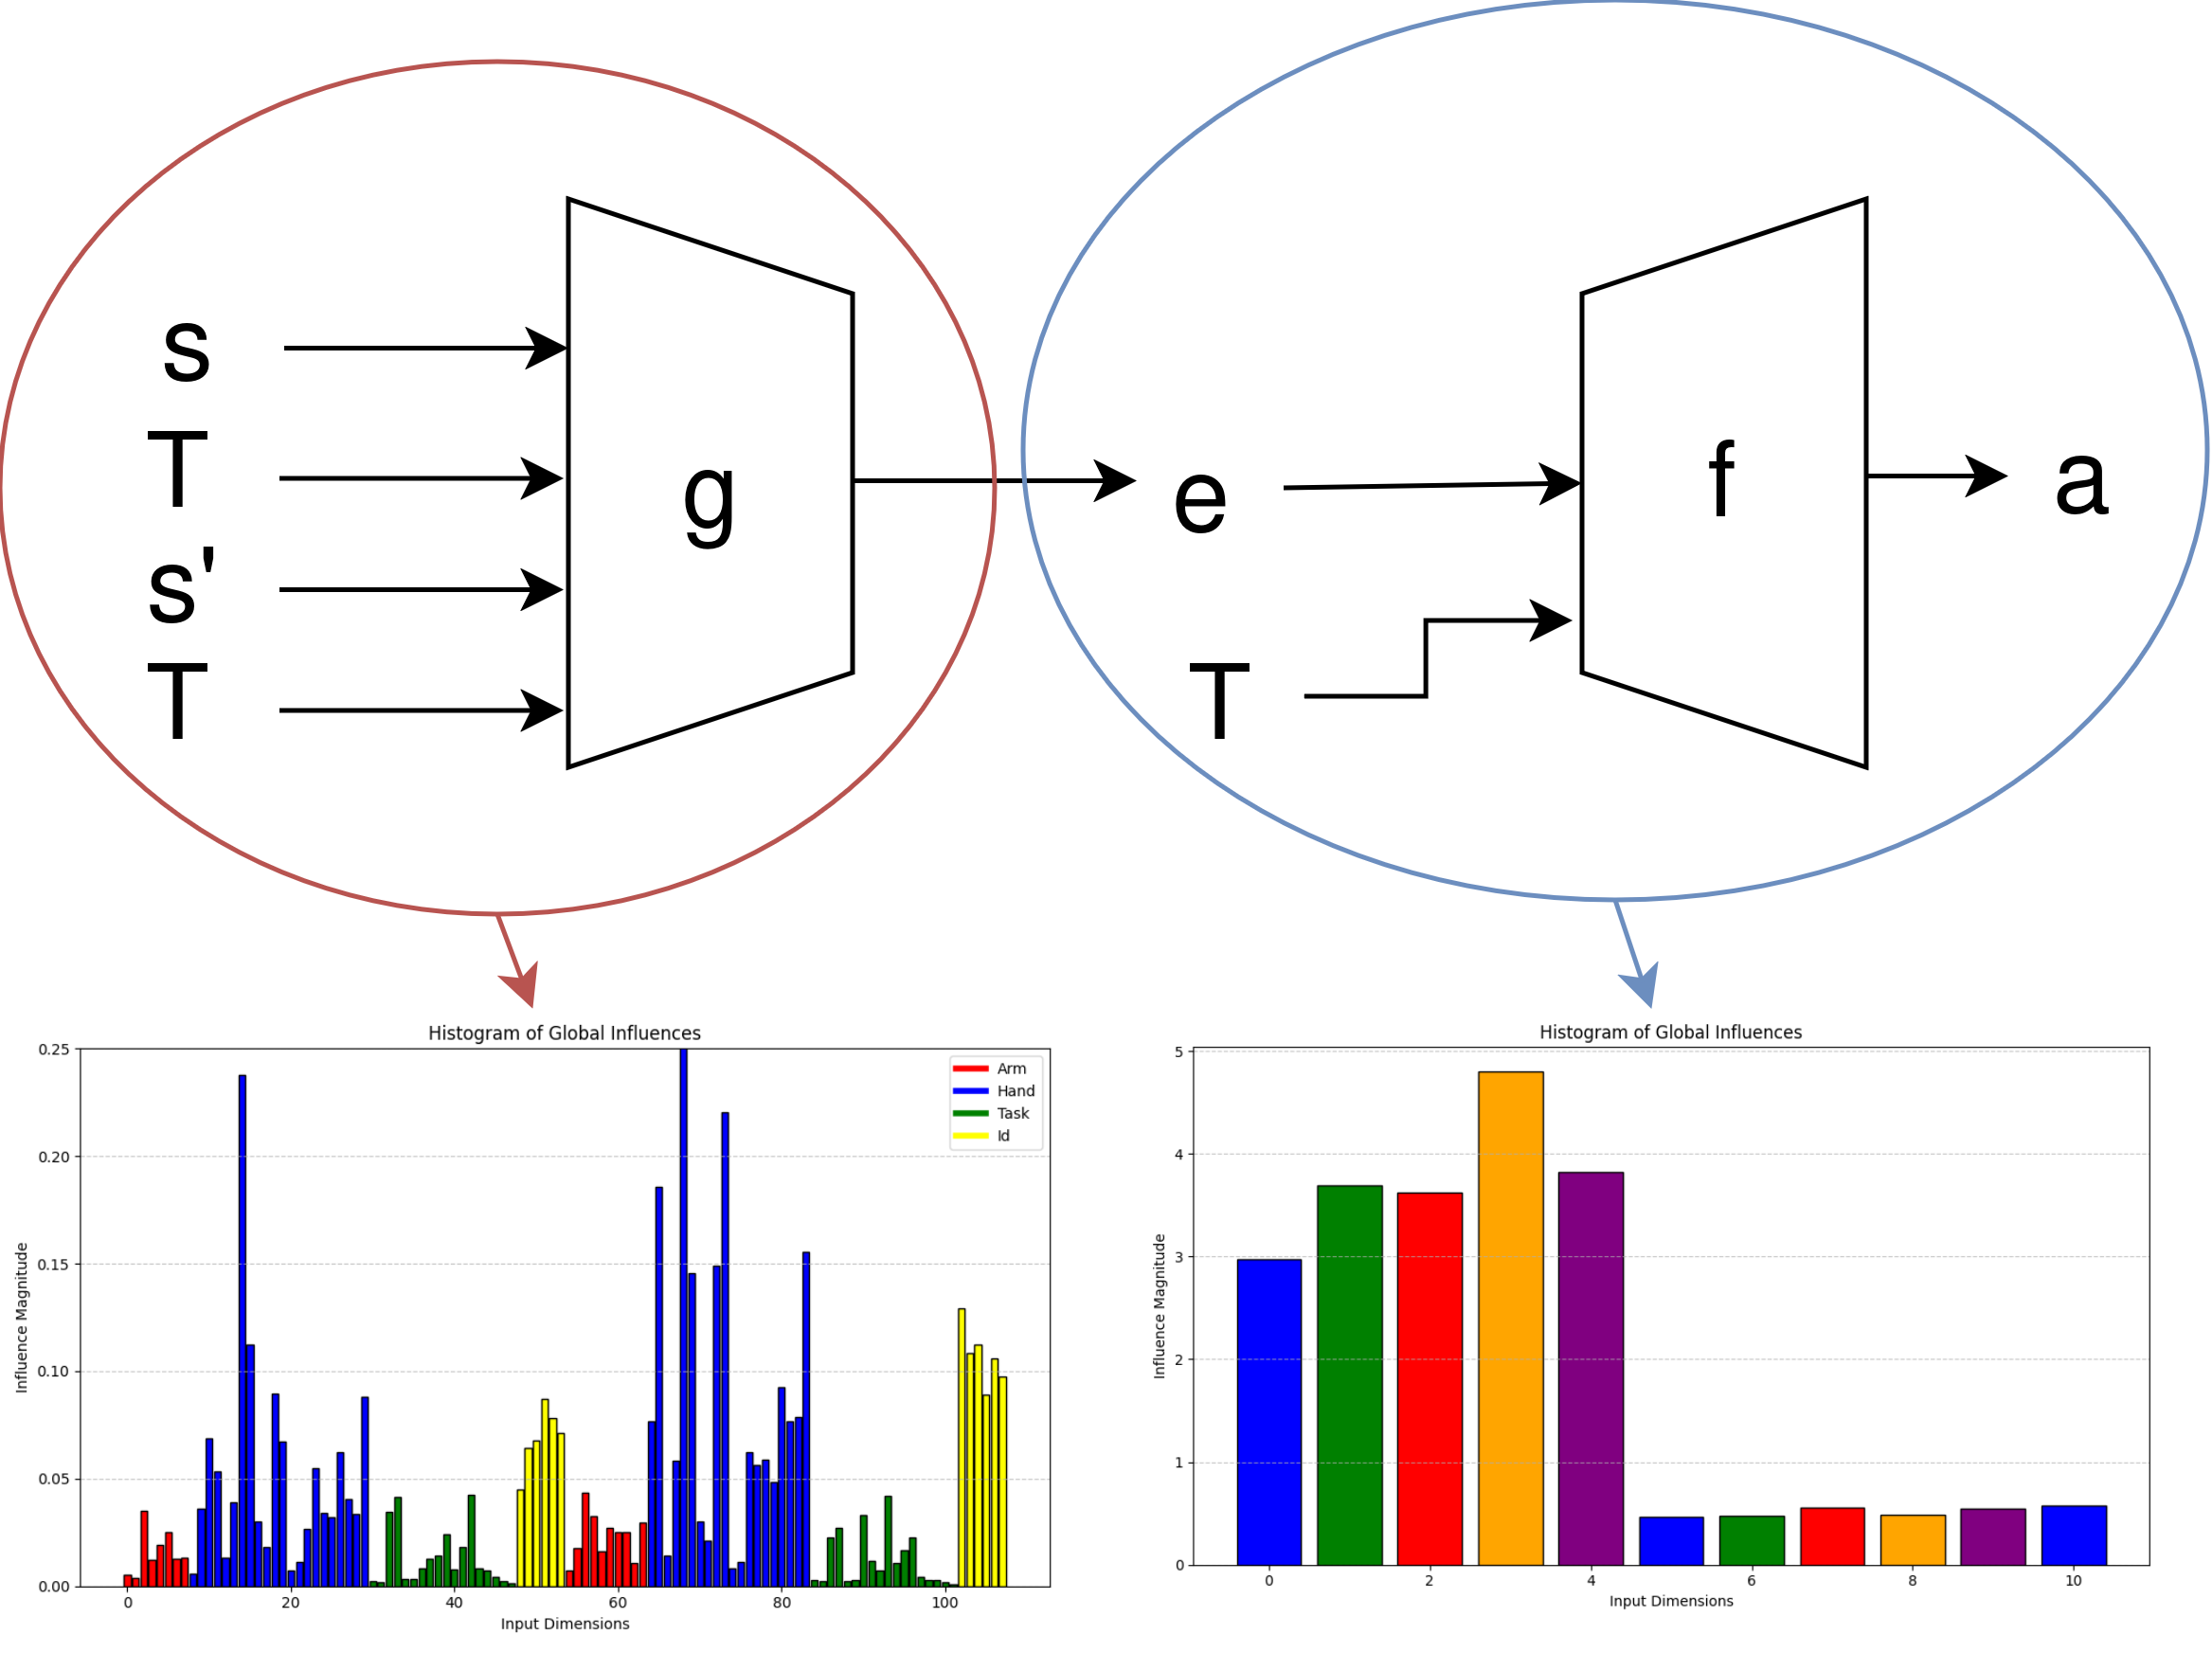
\includegraphics[width=0.8\textwidth]{img/sacaar_ig.png}
    \end{figure}
\end{frame}
\begin{frame}{Problema 3}
    Problema: As ações no dataset são independente das ações. O problema de exploração do SACAAR

    Solução: Melhorar a exploração permitindo sampling de ações fora da manifold. 

    \begin{figure}
        \begin{minipage}[t]{0.45\linewidth}
            \centering
            \vspace{0pt}
            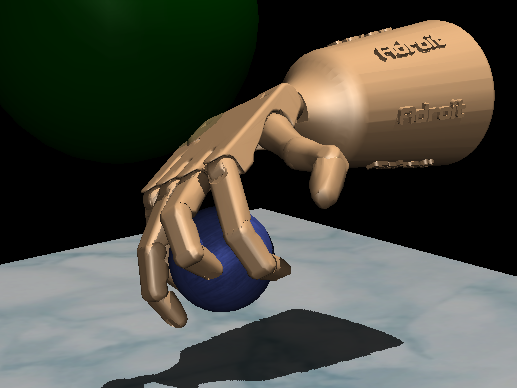
\includegraphics[width=\textwidth]{img/sphere.png}
        \end{minipage}
        \hspace{0.5cm}
        \begin{minipage}[t]{0.45\linewidth}
            \centering
            \vspace{0pt}
            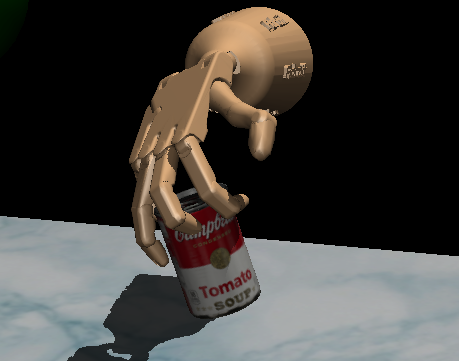
\includegraphics[width=\textwidth]{img/can.png}
        \end{minipage}
    \end{figure}
\end{frame}
\begin{frame}{Problema 3}
    Problema: As ações no dataset são independente das ações. O problema de exploração do SACAAR

    Solução: Melhorar a exploração permitindo sampling de ações fora da manifold. 

    \begin{figure}
        \centering
        \vspace{0pt}
        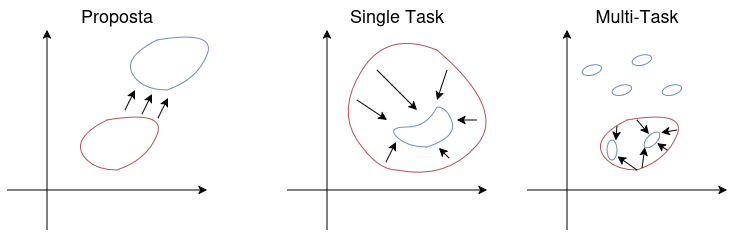
\includegraphics[width=\textwidth]{img/sacaar_exp.png}
    \end{figure}
\end{frame}
\begin{frame}{Problema 3}
    Problema: As ações no dataset são independente das ações. O problema de exploração do SACAAR

    Solução: Melhorar a exploração permitindo sampling de ações fora da manifold. 

    \begin{figure}
        \centering
        \vspace{0pt}
        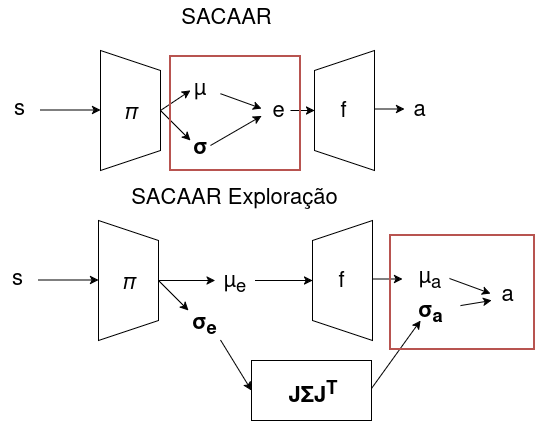
\includegraphics[width=0.65\textwidth]{img/sacaar_sigma.png}
    \end{figure}
\end{frame}
\begin{frame}{Problema 3}
    Problema: As ações no dataset são independente das ações. O problema de exploração do SACAAR

    Solução: Melhorar a exploração permitindo sampling de ações fora da manifold. 
    \begin{figure}
        \centering
        \vspace{-10pt}
        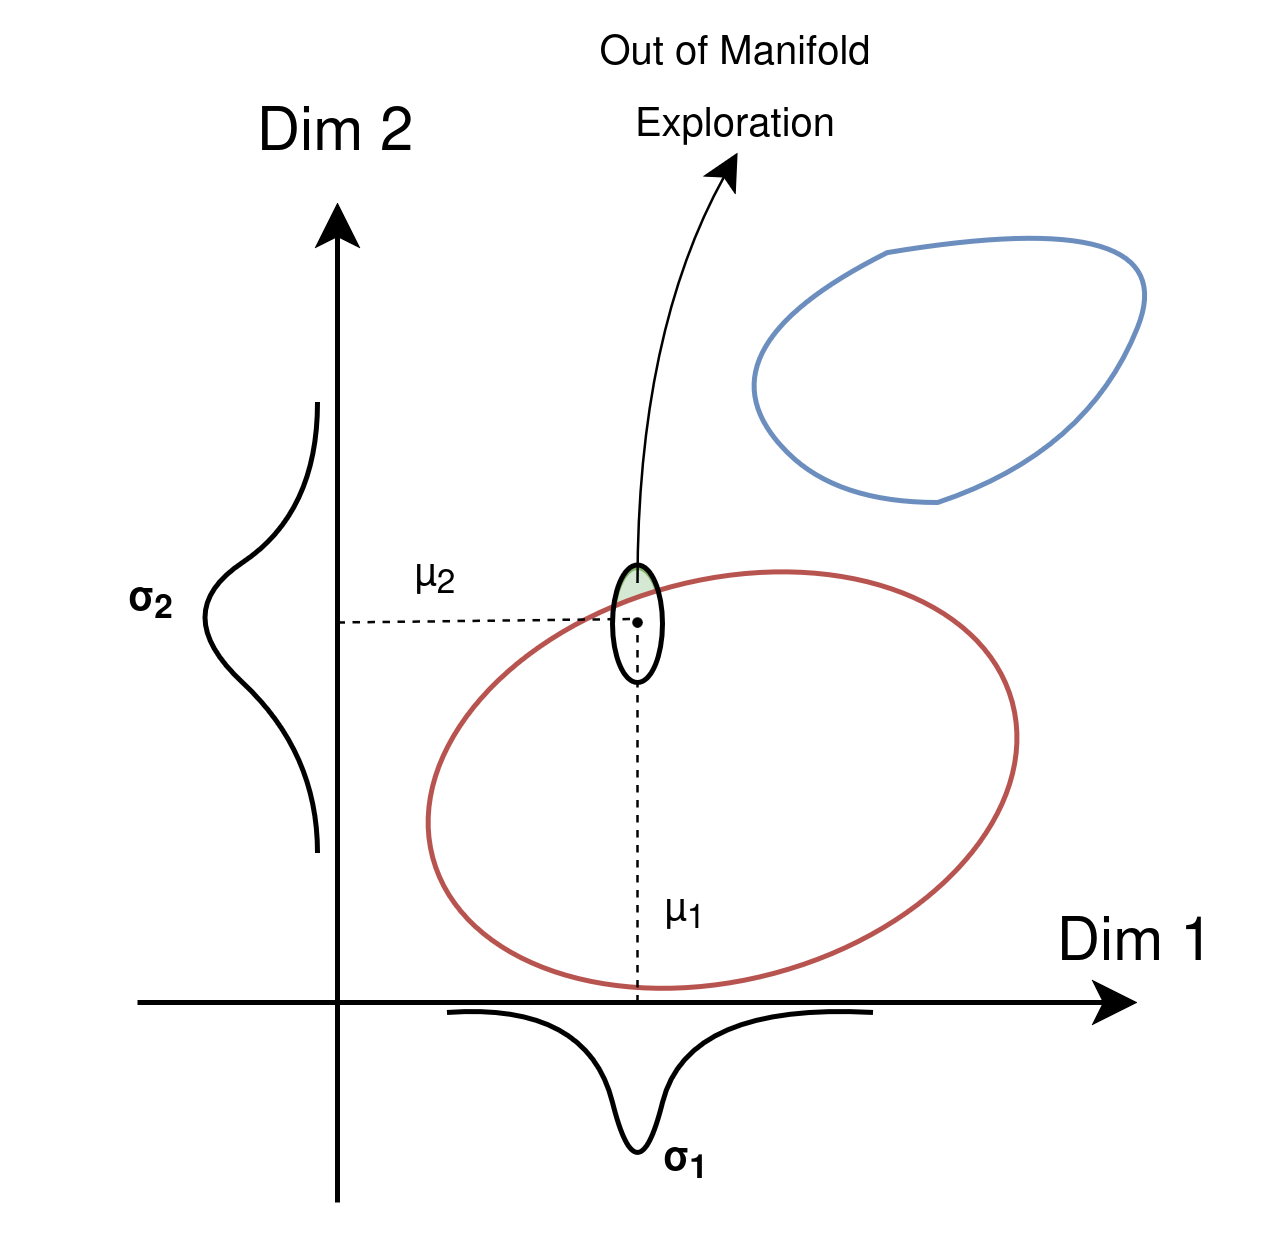
\includegraphics[width=0.6\textwidth]{img/sacaar_exp_man.png}
    \end{figure}
\end{frame}

\section{ML@UA}
\begin{frame}{ML@UA}
    \begin{figure}
        \centering
        
\includegraphics[width=0.3\textwidth]{img/white_space.png}
        \vspace{5cm}
        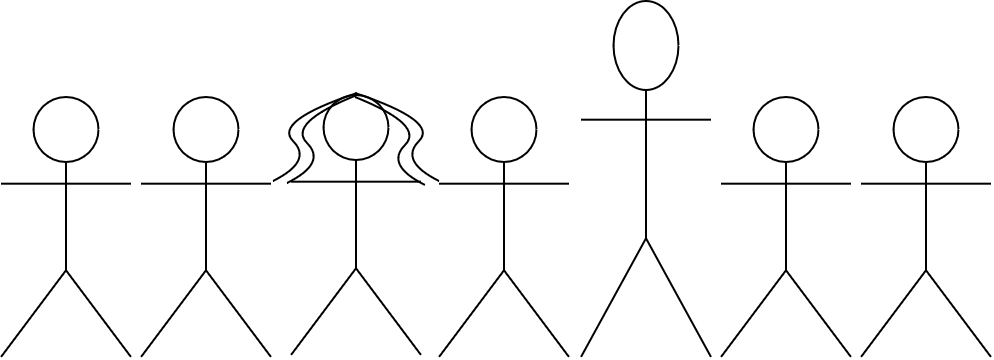
\includegraphics[width=0.75\textwidth]{img/ml-at-ua.png}
    \end{figure}
\end{frame}


\section{Kaggle competitions}
\begin{frame}{Kaggle competitions}
    \LARGE Group: Dr. Monkeys
    \vspace{29pt}
    \begin{figure}
        \centering
        \vspace{0pt}
        
\includegraphics[width=0.5\textwidth]{img/white_space.png}
    \end{figure}
\end{frame}
\begin{frame}{Kaggle competitions}
    \LARGE Group: Dr. Monkeys
    \vspace{10pt}
    \begin{figure}
        \centering
        \vspace{0pt}
        
\includegraphics[width=0.5\textwidth]{img/monkey-meme-simpson.jpg}
    \end{figure}
\end{frame}
\begin{frame}{Kaggle competitions}
    \begin{figure}
        \begin{minipage}[t]{0.30\linewidth}
            \centering
            \vspace{0pt}
            
\includegraphics[width=\textwidth]{img/kaggle.jpeg}
        \end{minipage}
        \hspace{0.5cm}
        \begin{minipage}[t]{0.50\linewidth}
            \centering
            \vspace{0pt}
            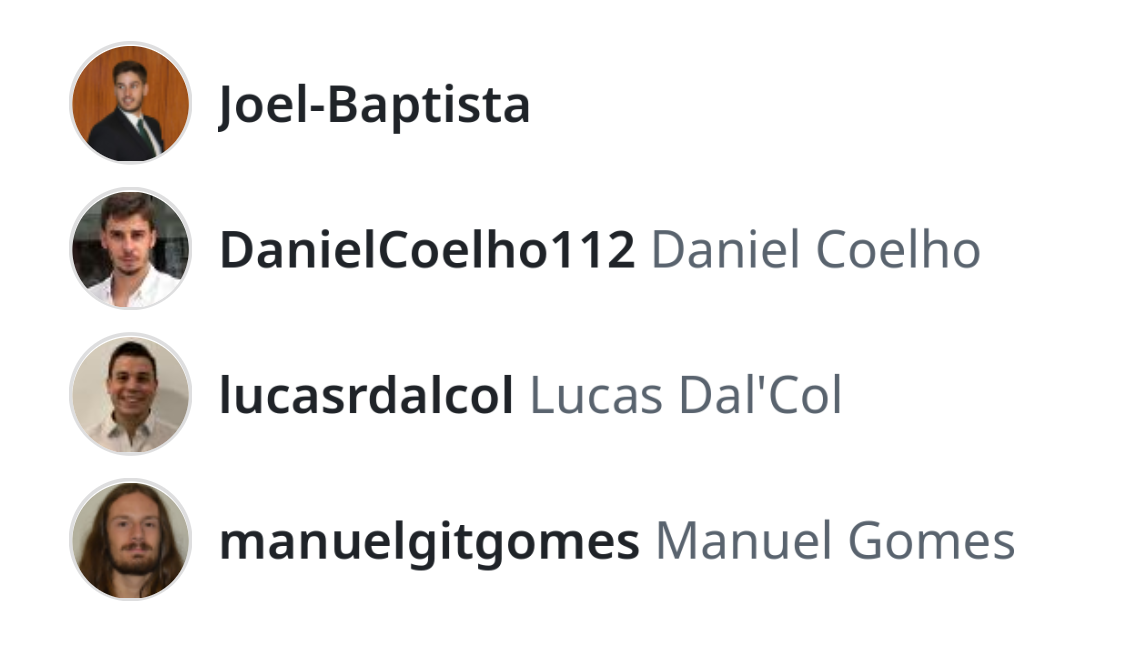
\includegraphics[width=\textwidth]{img/dr-monkeys.png}
        \end{minipage}
    \end{figure}
\end{frame}
\begin{frame}{Kaggle competitions}
    \begin{figure}
        \begin{minipage}[t]{\linewidth}
            \centering
            \vspace{0pt}
            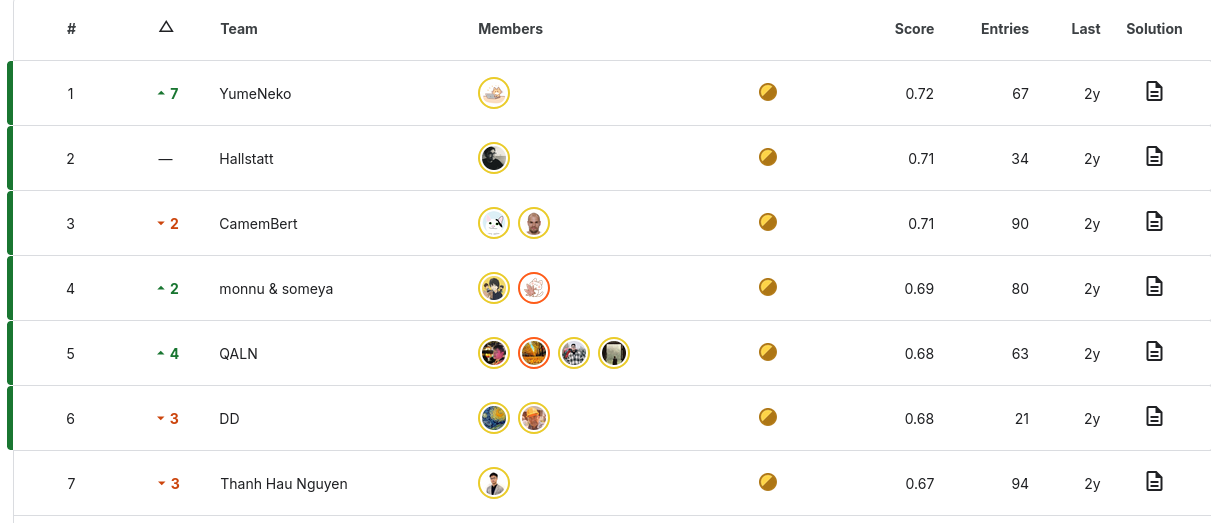
\includegraphics[width=\textwidth]{img/competition-2.png}
        \end{minipage}
        \vspace{0.5cm}
        \begin{minipage}[t]{\linewidth}
            \centering
            \vspace{0pt}
            
\includegraphics[width=\textwidth]{img/competition-1.png}
        \end{minipage}
    \end{figure}
\end{frame}

\section{Spring school}
\begin{frame}{Spring School}
    \begin{figure}
        \centering
        
\includegraphics[width=\textwidth]{img/INVICTA2024_banner.png}
    \end{figure}
\end{frame}
\begin{frame}{Spring School}
    \begin{figure}
        \centering
        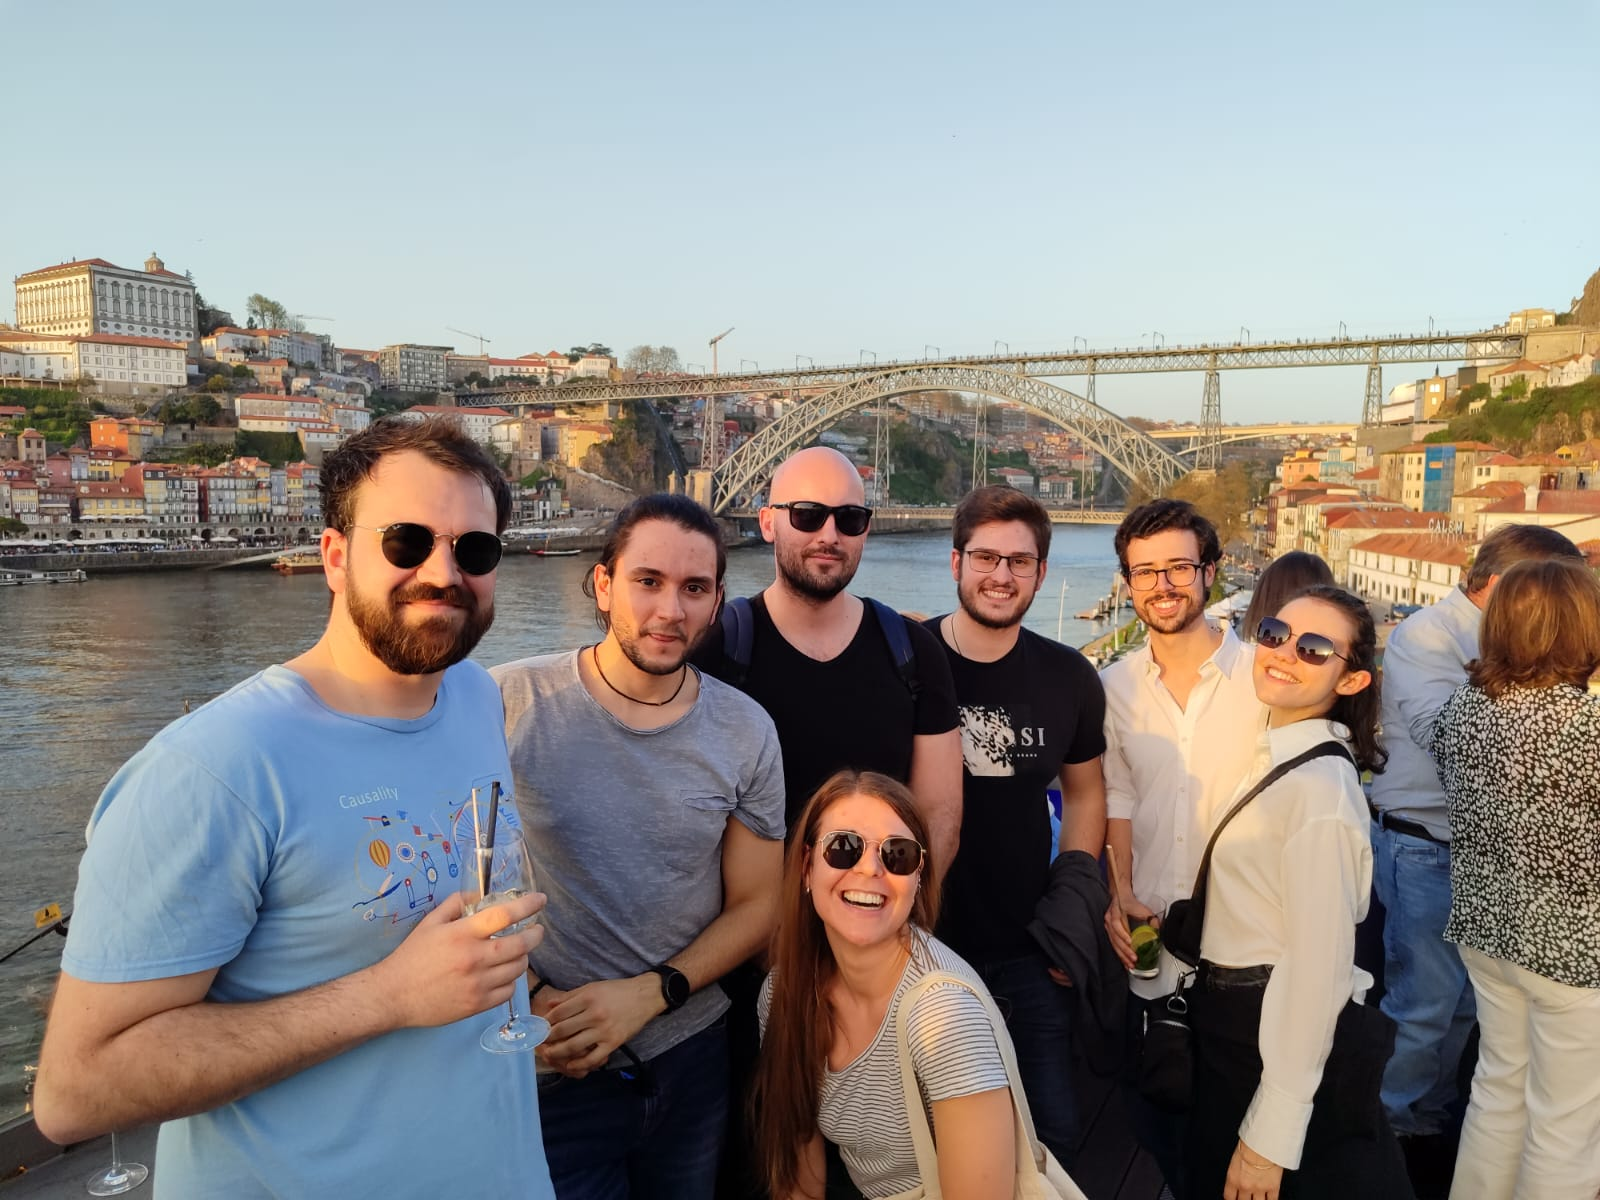
\includegraphics[width=0.75\textwidth]{img/invicta_group.jpeg}
    \end{figure}
\end{frame}


\section{Closing statement}
\begin{frame}{Conclusion}
    \center
    \LARGE
    Closing statement
\end{frame}



%%%%%%%%%%%%%%%%%%%%%%%%%%%%%%%%%%%%%%%%%%%%%%%%%%%%%%%%%%%

\end{document}


